\documentclass[paper=letter,11pt]{scrartcl}

\KOMAoptions{headinclude=true, footinclude=false}
\KOMAoptions{DIV=14, BCOR=5mm}
\KOMAoptions{numbers=noendperiod}
\KOMAoptions{parskip=half}
\addtokomafont{disposition}{\rmfamily}
\addtokomafont{part}{\LARGE}
\addtokomafont{descriptionlabel}{\rmfamily}
%\setkomafont{pageheadfoot}{\normalsize\sffamily}
\setkomafont{pagehead}{\normalsize\rmfamily}
%\setkomafont{publishers}{\normalsize\rmfamily}
\setkomafont{caption}{\normalfont\small}
\setcapindent{0pt}
\deffootnote[1em]{1em}{1em}{\textsuperscript{\thefootnotemark}\ }


\usepackage{amsmath}
\usepackage[varg]{txfonts}
\usepackage[T1]{fontenc}
\usepackage{graphicx}
\usepackage{xcolor}
\usepackage[american]{babel}
% hyperref is needed in many places, so include it here
\usepackage{hyperref}

\usepackage{xspace}
\usepackage{multirow}
\usepackage{float}


\usepackage{braket}
\usepackage{bbm}
\usepackage{relsize}
\usepackage{tcolorbox}

\def\ketY{\ensuremath{\ket {\Psi}}}
\def\iGeV{\ensuremath{\textrm{GeV}^{-1}}}
%\def\mp{\ensuremath{m_{\textrm{proton}}}}
\def\rp{\ensuremath{r_{\textrm{proton}}}}
\def\me{\ensuremath{m_{\textrm{electron}}}}
\def\aG{\ensuremath{\alpha_G}}
\def\rAtom{\ensuremath{r_{\textrm{atom}}}}
\def\rNucl{\ensuremath{r_{\textrm{nucleus}}}}
\def\GN{\ensuremath{\textrm{G}_\textrm{N}}}
\def\ketX{\ensuremath{\ket{\vec{x}}}}
\def\ve{\ensuremath{\vec{\epsilon}}}


\def\ABCDMatrix{\ensuremath{\begin{pmatrix} A &  B  \\ C  & D \end{pmatrix}}}
\def\xyprime{\ensuremath{\begin{pmatrix} x' \\ y' \end{pmatrix}}}
\def\xyprimeT{\ensuremath{\begin{pmatrix} x' &  y' \end{pmatrix}}}
\def\xy{\ensuremath{\begin{pmatrix} x \\ y \end{pmatrix}}}
\def\xyT{\ensuremath{\begin{pmatrix} x & y \end{pmatrix}}}

\def\IMatrix{\ensuremath{\begin{pmatrix} 0 &  1  \\ -1  & 0 \end{pmatrix}}}
\def\IBoostMatrix{\ensuremath{\begin{pmatrix} 0 &  1  \\ 1  & 0 \end{pmatrix}}}
\def\JThree{\ensuremath{\begin{pmatrix}    0 & -i & 0  \\ i & 0  & 0 \\ 0 & 0 & 0 \end{pmatrix}}} 
\def\JTwo{\ensuremath{\begin{bmatrix}    0 & 0 & -i  \\ 0 & 0  & 0 \\ i & 0 & 0 \end{bmatrix}}}
\def\JOne{\ensuremath{\begin{bmatrix}    0 & 0 & 0  \\ 0 & 0  & -i \\ 0 & i & 0 \end{bmatrix}}}
\def\etamn{\ensuremath{\eta_{\mu\nu}}}
\def\Lmn{\ensuremath{\Lambda^\mu_\nu}}
\def\dmn{\ensuremath{\delta^\mu_\nu}}
\def\wmn{\ensuremath{\omega^\mu_\nu}}
\def\be{\begin{equation*}}
\def\ee{\end{equation*}}
\def\bea{\begin{eqnarray*}}
\def\eea{\end{eqnarray*}}
\def\bi{\begin{itemize}}
\def\ei{\end{itemize}}
\def\fmn{\ensuremath{F_{\mu\nu}}}
\def\fMN{\ensuremath{F^{\mu\nu}}}
\def\bc{\begin{center}}
\def\ec{\end{center}}
\def\nus{$\nu$s}

\def\adagger{\ensuremath{a_{p\sigma}^\dagger}}
\def\lineacross{\noindent\rule{\textwidth}{1pt}}

\newcommand{\multiline}[1] {
\begin{tabular} {|l}
#1
\end{tabular}
}

\newcommand{\multilineNoLine}[1] {
\begin{tabular} {l}
#1
\end{tabular}
}



\newcommand{\lineTwo}[2] {
\begin{tabular} {|l}
#1 \\
#2
\end{tabular}
}

\newcommand{\rmt}[1] {
\textrm{#1}
}


%
% Units
%
\def\m{\ensuremath{\rmt{m}}}
\def\GeV{\ensuremath{\rmt{GeV}}}
\def\pt{\ensuremath{p_\rmt{T}}}


\def\parity{\ensuremath{\mathcal{P}}}

\usepackage{cancel}
\usepackage{ mathrsfs }
\def\bigL{\ensuremath{\mathscr{L}}}

\usepackage{ dsfont }



\usepackage{fancyhdr}
\fancyhf{}


\lhead{\Large 33-444} % \hfill Introduction to Particle Physics \hfill Spring 2019}
\chead{\Large Introduction to Particle Physics} % \hfill Spring 2019}
\rhead{\Large Spring 2019} % \hfill Introduction to Particle Physics \hfill Spring 2019}
\begin{document}
\thispagestyle{fancy}





%\begin{tabular}{c}
%{\large 33-444 \hfill Intro To Particle \hfill Spring 2019\\}
%\hline 
%\end{tabular}

\begin{center}
{\huge \textbf{Midterm}}
\large

\end{center}

{\large


\textbf{1) Why are energy and momentum conserved in the Standard Model ?  What would it mean if we found evidence for non-conservation of Energy ? What about non-conservation of Momentum? }\hfill \textit{(3 points)}\\

Physics is invariant to Space and time translations. 
These continuous symmetries lead to conserved currents via Noether's theorem.
The energy/momentum tensor is the associated conserved current. 

Non-conservation of energy would imply a violation of time translation invariance (eg: like in cosmology) 
Non-conservation of momentum would imply a violation of space translation invariance (eg: like near the surface of the earth)  

\vspace*{0.3in}

\textbf{2) What are three major consequences of combining QM and Relativity?}\hfill \textit{(3 points)}\\

Many possible answers, some I had in mind...\\
- Anti-particles\\
- Connection between spin and statistics\\
- Only contain certain types of leading interactions

\vspace*{0.3in}

\textbf{3) Muonic Atoms } \hfill \textit{(7 points)}\\
\begin{itemize}
\item[a)] The muon was the first elementary particle discovered that does not appear in ordinary atoms.  Negative muons can, however, form muonic atoms by replacing an electron in an ordinary atom. 
Estimate the size and binding energy of muonic hydrogen in GeV.

$m_\mu << m_p \Rightarrow $ to first order all motion in muon. 

\be
E\sim \frac{p^2}{m} - \frac{\alpha}{r} 
\ee


QM $\Rightarrow  p \sim \frac{1}{r}$ 


\be
E\sim \frac{1}{m_\mu r^2} - \frac{\alpha}{r} 
\ee

Equilibrium when terms are $\sim$ equal.

\be
\frac{1}{m_\mu r^2} = \frac{\alpha}{r} \Rightarrow r \sim \frac{1}{\alpha m_\mu} = 10^2\ 10^1\ GeV^{-1} = 10^3\ GeV^{-1}
\ee

Can get E from plugging this back into either of the two terms.

\be
E \sim \frac{\alpha}{r} \sim \alpha^2 m_\mu \sim 10^{-4}\ 10^{-1}\ GeV = 10^{-5}\ GeV
\ee

\item[b)] What is the ratio of the muonic hydrogen binding energy to that of regular hydrogen?

For regular hydrogen, same arguments as above with $m_\mu \rightarrow m_e$

$\Rightarrow$

\be
\frac{E^\mu}{E^e} = \frac{\alpha^2 m_\mu}{\alpha^2 m_e} =  \frac{m_\mu}{m_e}
\ee

\end{itemize}


\textbf{4) Why do we label particle states by momentum? } \hfill \textit{(2 points)}\\

B/c translations are a good symmetry and momentum states transform nicely under translations.



\textbf{5) What are two restrictions to particle interactions that are a consequence gauge invariance ? }\hfill \textit{(2 points)}\\

Again there are many, here are a few that I have in mind.\\
-) Charge conservation\\
-) Principle of equivalence\\
-) Massless Spin-1 particles have to couple to particles of the same mass\\
-) Cannot have massless interacting particles with spin > 2.

\textbf{6) Lorentz Transforms } \hfill \textit{(4 points)}\\
\begin{itemize}
\item[a)] How does a \textbf{massive} particle $\ket{p^\mu,\sigma}$ transform under a little group transformation ($W_\mu^\nu$)  ?
$W_\mu^\nu \ket{p^\mu,\sigma} = \sum_{\sigma'} R_{\sigma \sigma'} \ket{p^\mu,\sigma'}$, where R is a rotation matrix.
\item[b)] How does a \textbf{massless} particle $\ket{p^\mu,\sigma}$ transform under a little group transformation ($W_\mu^\nu$)  ?
$W_\mu^\nu \ket{p^\mu,\sigma} = e^{ih\theta} \ket{p^\mu,\sigma'}$, where h is the particles helicity.
\item[c)] How does a \textbf{massive} particle $\ket{p^\mu,\sigma}$ transform under a general Lorentz transformation ($\Lambda_\mu^\nu$) ?
$\Lambda_\mu^\nu \ket{p^\mu,\sigma} = \sum_{\sigma'} R_{\sigma \sigma'} \ket{\Lambda p,\sigma'}$, where R is a rotation matrix.
\item[d)] How does a \textbf{massless} particle $\ket{p^\mu,\sigma}$ transform under a general Lorentz transformation ($\Lambda_\mu^\nu$)?
$\Lambda_\mu^\nu \ket{p^\mu,\sigma} = e^{ih\theta} \ket{\Lambda p,\sigma'}$, where h is the particles helicity.
\end{itemize}


\textbf{7) Can the SM have interactions between fermions and massless particles with Spin 2 ? If not, why not.  What about interactions between mass-less Spin 3 particles and fermions ? If not, why not. }\hfill \textit{(2 points)}\\

\bc
Spin 2 yes (But the coupling is universal)\\
Spin 3 no
\ec

\textbf{8) Yukawa’s Theory.}\hfill \textit{(2 points)}
In the 1930s, Hideki Yukawa predicted the existence of a new particle, now called the pion, which is responsible for binding protons and neutrons together in atomic nuclei. 
Estimate the mass of the pion from the assumed range of the force. ($10^{-15}$ meters). 
Express the mass in GeV.

\be
10^{-15} m \sim \GeV^{-1} \Rightarrow m_\pi \sim  \GeV
\ee


\textbf{9)  How many generators does the Lorentz group have ? }\hfill \textit{(3 points)}\\
What transformations do they correspond to ?

\bc
6:  3-rotations about x,y,z  and 3 boosts along x,y,and z
\ec


\textbf{10) Fields } \hfill \textit{(2 points)}\\
In QFT why do we write interactions in terms of fields (Fourier transforms of creation and annihilation operators)  instead  of the creation and annihilation operators directly?

\bc
Locality.
\ec


\textbf{11) Why is the weak interaction so much weaker than then electromagnetic interactions at low energies? } \hfill \textit{(2 points)}\\

\bc
Massive force carriers
\ec

\clearpage

\textbf{12) Lagrangians } \hfill \textit{(3 points)}\\
Consider the following Lagrangian:
\be
L = \frac{1}{2} (\partial_\mu\phi)(\partial^\mu\phi) - \frac{m^2}{2}\phi^2 + \bar{\psi}[i\gamma_\mu\partial^\mu]\psi + g_1 \phi \psi \psi + g_2 \psi \psi \psi \psi + g_3 \phi \phi \phi \phi
\ee

\bc
All terms must have mass dimension 4. Bosons like $\phi$ have mass dimension 1. Fermions like $\psi$ have mass dimension $\frac{3}{2}$.  These you could deduce from the kinetic (bilinear) terms.
\ec

\bi
\item[a)] What is the dimension of $g_1$ ?   dimension-less 

\item[b)] What is the dimension of $g_2$ ?  $m^{-2}$
  
\item[c)] What is the dimension of $g_3$ ?  dimension-less 

\ei


\textbf{13) Feynman Diagrams }\hfill \textit{(15 points)}\\
Fermions of type $x$ scatter into fermions of type $y$ through the diagram shown below, where $S$ is a massive scalar. 
At low energies ($P_x P_y << m_S$) the cross section for this process is given by $\sigma_0$.
Assume $m_x$ and $m_y$ are both negligible. 
\bc
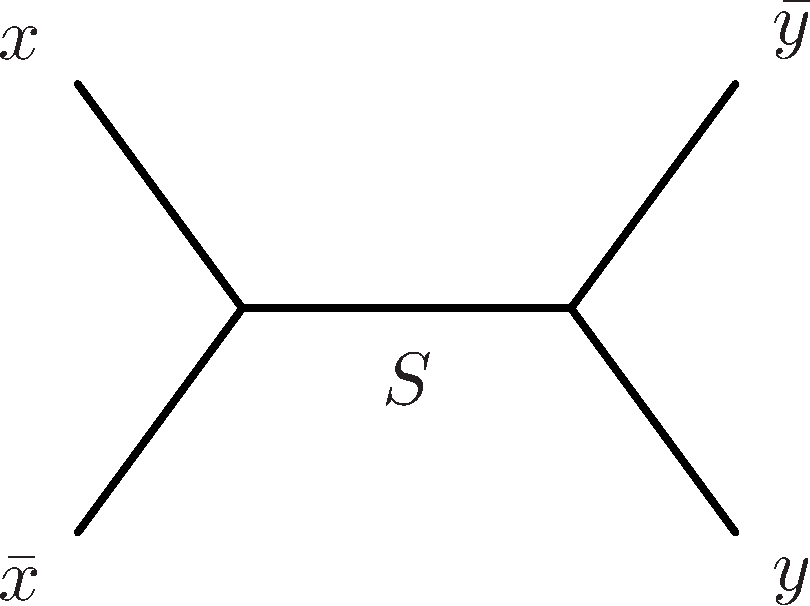
\includegraphics[width=0.2\textwidth]{./xxToyy.pdf}
\ec
\bi
\item[a)] How does this cross section change if the ``S-charge'' of the $x$ particle is doubled ? \\ (S-charge being the $x\bar{x} \rightarrow S$ coupling) 

\be
\sigma \sim |M|^2 \hspace*{0.5in} M \sim q_s
\ee

\be
q_s\rightarrow 2q_s \Rightarrow M \rightarrow 2M \Rightarrow \sigma \rightarrow 4\sigma
\ee


\item[b)] How does the cross section change if the mass of the $S$-particle is doubled ?

\be
\sigma \sim |M|^2 \hspace*{0.5in} M \sim \frac{1}{M_S^2}
\ee

\be
M_S\rightarrow 2M_S \Rightarrow M \rightarrow \frac{1}{4}M \Rightarrow \sigma \rightarrow \frac{1}{16}\sigma
\ee


\item[c)] At low energies, how does the cross section depend on the center of mass energy of the scattering $E_{CM}$ ? 
\textit{(Hint: At low energies you can think of the $xx \rightarrow yy$ scattering as described by an effective 4-point $xxyy$ interaction, as Fermi did for neutrino scattering.)}

At low energies the scattering is described by an effective 4-point $xxyyy$ interaction.
The xxyy vertex has 4 fermions which each have mass dimension $\frac{3}{2}$.  
So the diagram has mass dimension $[g_{xxyy}] 4 \times \frac{3}{2} = [g_{xxyy}] \times 6$. 
In order to have overall mass dimension four, the mass dimension of the coupling $[g_{xxyy}]$ must be $\GeV^{-2}$.

\be
M \sim \GeV^{-2} \Rightarrow |M|^2 \sim \GeV^{-4}
\ee

Dimensions of $\sigma$ have to work out to be $\GeV^{-2}$.

The only other energy scale in the problem is $E_{CM}$ so.

\be
\sigma \sim \frac{E_{CM}^2}{\GeV^{4}}
\ee

%the four-point $xx\rightarrow yy$ scattering diagram has a coupling constant with mass dimensiton $GeV^{-2}$.



\ei





\clearpage



} % Begning Large
\end{document}
